\documentclass[12pt,a4paper,]{book}
\def\ifdoblecara{} %% set to true
\def\ifprincipal{} %% set to true
\let\ifprincipal\undefined %% set to false
\def\ifcitapandoc{} %% set to true
\let\ifcitapandoc\undefined %% set to false
\usepackage{lmodern}
% sin fontmathfamily
\usepackage{amssymb,amsmath}
\usepackage{ifxetex,ifluatex}
%\usepackage{fixltx2e} % provides \textsubscript %PLLC
\ifnum 0\ifxetex 1\fi\ifluatex 1\fi=0 % if pdftex
  \usepackage[T1]{fontenc}
  \usepackage[utf8]{inputenc}
\else % if luatex or xelatex
  \ifxetex
    \usepackage{mathspec}
  \else
    \usepackage{fontspec}
  \fi
  \defaultfontfeatures{Ligatures=TeX,Scale=MatchLowercase}
\fi
% use upquote if available, for straight quotes in verbatim environments
\IfFileExists{upquote.sty}{\usepackage{upquote}}{}
% use microtype if available
\IfFileExists{microtype.sty}{%
\usepackage{microtype}
\UseMicrotypeSet[protrusion]{basicmath} % disable protrusion for tt fonts
}{}
\usepackage[margin = 2.5cm]{geometry}
\usepackage{hyperref}
\hypersetup{unicode=true,
            pdfauthor={Nombre Completo Autor},
              pdfborder={0 0 0},
              breaklinks=true}
\urlstyle{same}  % don't use monospace font for urls
%
\usepackage[usenames,dvipsnames]{xcolor}  %new PLLC
\IfFileExists{parskip.sty}{%
\usepackage{parskip}
}{% else
\setlength{\parindent}{0pt}
\setlength{\parskip}{6pt plus 2pt minus 1pt}
}
\setlength{\emergencystretch}{3em}  % prevent overfull lines
\providecommand{\tightlist}{%
  \setlength{\itemsep}{0pt}\setlength{\parskip}{0pt}}
\setcounter{secnumdepth}{5}
% Redefines (sub)paragraphs to behave more like sections
\ifx\paragraph\undefined\else
\let\oldparagraph\paragraph
\renewcommand{\paragraph}[1]{\oldparagraph{#1}\mbox{}}
\fi
\ifx\subparagraph\undefined\else
\let\oldsubparagraph\subparagraph
\renewcommand{\subparagraph}[1]{\oldsubparagraph{#1}\mbox{}}
\fi

%%% Use protect on footnotes to avoid problems with footnotes in titles
\let\rmarkdownfootnote\footnote%
\def\footnote{\protect\rmarkdownfootnote}


  \title{}
    \author{Nombre Completo Autor}
      \date{18/11/2021}


%%%%%%% inicio: latex_preambulo.tex PLLC


%% UTILIZA CODIFICACIÓN UTF-8
%% MODIFICARLO CONVENIENTEMENTE PARA USARLO CON OTRAS CODIFICACIONES


%\usepackage[spanish,es-nodecimaldot,es-noshorthands]{babel}
\usepackage[spanish,es-nodecimaldot,es-noshorthands,es-tabla]{babel}
% Ver: es-tabla (en: https://osl.ugr.es/CTAN/macros/latex/contrib/babel-contrib/spanish/spanish.pdf)
% es-tabla (en: https://tex.stackexchange.com/questions/80443/change-the-word-table-in-table-captions)
\usepackage[spanish, plain, datebegin,sortcompress,nocomment,
noabstract]{flexbib}
 
\usepackage{float}
\usepackage{placeins}
\usepackage{fancyhdr}
% Solucion: ! LaTeX Error: Command \counterwithout already defined.
% https://tex.stackexchange.com/questions/425600/latex-error-command-counterwithout-already-defined
\let\counterwithout\relax
\let\counterwithin\relax
\usepackage{chngcntr}
%\usepackage{microtype}  %antes en template PLLC
\usepackage[utf8]{inputenc}
\usepackage[T1]{fontenc} % Usa codificación 8-bit que tiene 256 glyphs

%\usepackage[dvipsnames]{xcolor}
%\usepackage[usenames,dvipsnames]{xcolor}  %new
\usepackage{pdfpages}
%\usepackage{natbib}




% Para portada: latex_paginatitulo_mod_ST02.tex (inicio)
\usepackage{tikz}
\usepackage{epigraph}
\input{portadas/latex_paginatitulo_mod_ST02_add.sty}
% Para portada: latex_paginatitulo_mod_ST02.tex (fin)

% Para portada: latex_paginatitulo_mod_OV01.tex (inicio)
\usepackage{cpimod}
% Para portada: latex_paginatitulo_mod_OV01.tex (fin)

% Para portada: latex_paginatitulo_mod_OV03.tex (inicio)
\usepackage{KTHEEtitlepage}
% Para portada: latex_paginatitulo_mod_OV03.tex (fin)

\renewcommand{\contentsname}{Índice}
\renewcommand{\listfigurename}{Índice de figuras}
\renewcommand{\listtablename}{Índice de tablas}
\newcommand{\bcols}{}
\newcommand{\ecols}{}
\newcommand{\bcol}[1]{\begin{minipage}{#1\linewidth}}
\newcommand{\ecol}{\end{minipage}}
\newcommand{\balertblock}[1]{\begin{alertblock}{#1}}
\newcommand{\ealertblock}{\end{alertblock}}
\newcommand{\bitemize}{\begin{itemize}}
\newcommand{\eitemize}{\end{itemize}}
\newcommand{\benumerate}{\begin{enumerate}}
\newcommand{\eenumerate}{\end{enumerate}}
\newcommand{\saltopagina}{\newpage}
\newcommand{\bcenter}{\begin{center}}
\newcommand{\ecenter}{\end{center}}
\newcommand{\beproof}{\begin{proof}} %new
\newcommand{\eeproof}{\end{proof}} %new
%De: https://texblog.org/2007/11/07/headerfooter-in-latex-with-fancyhdr/
% \fancyhead
% E: Even page
% O: Odd page
% L: Left field
% C: Center field
% R: Right field
% H: Header
% F: Footer
%\fancyhead[CO,CE]{Resultados}

%OPCION 1
% \fancyhead[LE,RO]{\slshape \rightmark}
% \fancyhead[LO,RE]{\slshape \leftmark}
% \fancyfoot[C]{\thepage}
% \renewcommand{\headrulewidth}{0.4pt}
% \renewcommand{\footrulewidth}{0pt}

%OPCION 2
% \fancyhead[LE,RO]{\slshape \rightmark}
% \fancyfoot[LO,RE]{\slshape \leftmark}
% \fancyfoot[LE,RO]{\thepage}
% \renewcommand{\headrulewidth}{0.4pt}
% \renewcommand{\footrulewidth}{0.4pt}
%%%%%%%%%%
\usepackage{calc,amsfonts}
% Elimina la cabecera de páginas impares vacías al finalizar los capítulos
\usepackage{emptypage}
\makeatletter

%\definecolor{ocre}{RGB}{25,25,243} % Define el color azul (naranja) usado para resaltar algunas salidas
\definecolor{ocre}{RGB}{0,0,0} % Define el color a negro (aparece en los teoremas

%\usepackage{calc} 


%era if(csl-refs) con dolares
% metodobib: true


\usepackage{lipsum}

%\usepackage{tikz} % Requerido para dibujar formas personalizadas

%\usepackage{amsmath,amsthm,amssymb,amsfonts}
\usepackage{amsthm}


% Boxed/framed environments
\newtheoremstyle{ocrenumbox}% % Theorem style name
{0pt}% Space above
{0pt}% Space below
{\normalfont}% % Body font
{}% Indent amount
{\small\bf\sffamily\color{ocre}}% % Theorem head font
{\;}% Punctuation after theorem head
{0.25em}% Space after theorem head
{\small\sffamily\color{ocre}\thmname{#1}\nobreakspace\thmnumber{\@ifnotempty{#1}{}\@upn{#2}}% Theorem text (e.g. Theorem 2.1)
\thmnote{\nobreakspace\the\thm@notefont\sffamily\bfseries\color{black}---\nobreakspace#3.}} % Optional theorem note
\renewcommand{\qedsymbol}{$\blacksquare$}% Optional qed square

\newtheoremstyle{blacknumex}% Theorem style name
{5pt}% Space above
{5pt}% Space below
{\normalfont}% Body font
{} % Indent amount
{\small\bf\sffamily}% Theorem head font
{\;}% Punctuation after theorem head
{0.25em}% Space after theorem head
{\small\sffamily{\tiny\ensuremath{\blacksquare}}\nobreakspace\thmname{#1}\nobreakspace\thmnumber{\@ifnotempty{#1}{}\@upn{#2}}% Theorem text (e.g. Theorem 2.1)
\thmnote{\nobreakspace\the\thm@notefont\sffamily\bfseries---\nobreakspace#3.}}% Optional theorem note

\newtheoremstyle{blacknumbox} % Theorem style name
{0pt}% Space above
{0pt}% Space below
{\normalfont}% Body font
{}% Indent amount
{\small\bf\sffamily}% Theorem head font
{\;}% Punctuation after theorem head
{0.25em}% Space after theorem head
{\small\sffamily\thmname{#1}\nobreakspace\thmnumber{\@ifnotempty{#1}{}\@upn{#2}}% Theorem text (e.g. Theorem 2.1)
\thmnote{\nobreakspace\the\thm@notefont\sffamily\bfseries---\nobreakspace#3.}}% Optional theorem note

% Non-boxed/non-framed environments
\newtheoremstyle{ocrenum}% % Theorem style name
{5pt}% Space above
{5pt}% Space below
{\normalfont}% % Body font
{}% Indent amount
{\small\bf\sffamily\color{ocre}}% % Theorem head font
{\;}% Punctuation after theorem head
{0.25em}% Space after theorem head
{\small\sffamily\color{ocre}\thmname{#1}\nobreakspace\thmnumber{\@ifnotempty{#1}{}\@upn{#2}}% Theorem text (e.g. Theorem 2.1)
\thmnote{\nobreakspace\the\thm@notefont\sffamily\bfseries\color{black}---\nobreakspace#3.}} % Optional theorem note
\renewcommand{\qedsymbol}{$\blacksquare$}% Optional qed square
\makeatother



% Define el estilo texto theorem para cada tipo definido anteriormente
\newcounter{dummy} 
\numberwithin{dummy}{section}
\theoremstyle{ocrenumbox}
\newtheorem{theoremeT}[dummy]{Teorema}  % (Pedro: Theorem)
\newtheorem{problem}{Problema}[chapter]  % (Pedro: Problem)
\newtheorem{exerciseT}{Ejercicio}[chapter] % (Pedro: Exercise)
\theoremstyle{blacknumex}
\newtheorem{exampleT}{Ejemplo}[chapter] % (Pedro: Example)
\theoremstyle{blacknumbox}
\newtheorem{vocabulary}{Vocabulario}[chapter]  % (Pedro: Vocabulary)
\newtheorem{definitionT}{Definición}[section]  % (Pedro: Definition)
\newtheorem{corollaryT}[dummy]{Corolario}  % (Pedro: Corollary)
\theoremstyle{ocrenum}
\newtheorem{proposition}[dummy]{Proposición} % (Pedro: Proposition)


\usepackage[framemethod=default]{mdframed}



\newcommand{\intoo}[2]{\mathopen{]}#1\,;#2\mathclose{[}}
\newcommand{\ud}{\mathop{\mathrm{{}d}}\mathopen{}}
\newcommand{\intff}[2]{\mathopen{[}#1\,;#2\mathclose{]}}
\newtheorem{notation}{Notation}[chapter]


\mdfdefinestyle{exampledefault}{%
rightline=true,innerleftmargin=10,innerrightmargin=10,
frametitlerule=true,frametitlerulecolor=green,
frametitlebackgroundcolor=yellow,
frametitlerulewidth=2pt}


% Theorem box
\newmdenv[skipabove=7pt,
skipbelow=7pt,
backgroundcolor=black!5,
linecolor=ocre,
innerleftmargin=5pt,
innerrightmargin=5pt,
innertopmargin=10pt,%5pt
leftmargin=0cm,
rightmargin=0cm,
innerbottommargin=5pt]{tBox}

% Exercise box	  
\newmdenv[skipabove=7pt,
skipbelow=7pt,
rightline=false,
leftline=true,
topline=false,
bottomline=false,
backgroundcolor=ocre!10,
linecolor=ocre,
innerleftmargin=5pt,
innerrightmargin=5pt,
innertopmargin=10pt,%5pt
innerbottommargin=5pt,
leftmargin=0cm,
rightmargin=0cm,
linewidth=4pt]{eBox}	

% Definition box
\newmdenv[skipabove=7pt,
skipbelow=7pt,
rightline=false,
leftline=true,
topline=false,
bottomline=false,
linecolor=ocre,
innerleftmargin=5pt,
innerrightmargin=5pt,
innertopmargin=10pt,%0pt
leftmargin=0cm,
rightmargin=0cm,
linewidth=4pt,
innerbottommargin=0pt]{dBox}	

% Corollary box
\newmdenv[skipabove=7pt,
skipbelow=7pt,
rightline=false,
leftline=true,
topline=false,
bottomline=false,
linecolor=gray,
backgroundcolor=black!5,
innerleftmargin=5pt,
innerrightmargin=5pt,
innertopmargin=10pt,%5pt
leftmargin=0cm,
rightmargin=0cm,
linewidth=4pt,
innerbottommargin=5pt]{cBox}

% Crea un entorno para cada tipo de theorem y le asigna un estilo 
% con ayuda de las cajas coloreadas anteriores
\newenvironment{theorem}{\begin{tBox}\begin{theoremeT}}{\end{theoremeT}\end{tBox}}
\newenvironment{exercise}{\begin{eBox}\begin{exerciseT}}{\hfill{\color{ocre}\tiny\ensuremath{\blacksquare}}\end{exerciseT}\end{eBox}}				  
\newenvironment{definition}{\begin{dBox}\begin{definitionT}}{\end{definitionT}\end{dBox}}	
\newenvironment{example}{\begin{exampleT}}{\hfill{\tiny\ensuremath{\blacksquare}}\end{exampleT}}		
\newenvironment{corollary}{\begin{cBox}\begin{corollaryT}}{\end{corollaryT}\end{cBox}}	

%	ENVIRONMENT remark
\newenvironment{remark}{\par\vspace{10pt}\small 
% Espacio blanco vertical sobre la nota y tamaño de fuente menor
\begin{list}{}{
\leftmargin=35pt % Indentación sobre la izquierda
\rightmargin=25pt}\item\ignorespaces % Indentación sobre la derecha
\makebox[-2.5pt]{\begin{tikzpicture}[overlay]
\node[draw=ocre!60,line width=1pt,circle,fill=ocre!25,font=\sffamily\bfseries,inner sep=2pt,outer sep=0pt] at (-15pt,0pt){\textcolor{ocre}{N}}; \end{tikzpicture}} % R naranja en un círculo (Pedro)
\advance\baselineskip -1pt}{\end{list}\vskip5pt} 
% Espaciado de línea más estrecho y espacio en blanco después del comentario


\newenvironment{solutionExe}{\par\vspace{10pt}\small 
\begin{list}{}{
\leftmargin=35pt 
\rightmargin=25pt}\item\ignorespaces 
\makebox[-2.5pt]{\begin{tikzpicture}[overlay]
\node[draw=ocre!60,line width=1pt,circle,fill=ocre!25,font=\sffamily\bfseries,inner sep=2pt,outer sep=0pt] at (-15pt,0pt){\textcolor{ocre}{S}}; \end{tikzpicture}} 
\advance\baselineskip -1pt}{\end{list}\vskip5pt} 

\newenvironment{solutionExa}{\par\vspace{10pt}\small 
\begin{list}{}{
\leftmargin=35pt 
\rightmargin=25pt}\item\ignorespaces 
\makebox[-2.5pt]{\begin{tikzpicture}[overlay]
\node[draw=ocre!60,line width=1pt,circle,fill=ocre!55,font=\sffamily\bfseries,inner sep=2pt,outer sep=0pt] at (-15pt,0pt){\textcolor{ocre}{S}}; \end{tikzpicture}} 
\advance\baselineskip -1pt}{\end{list}\vskip5pt} 

\usepackage{tcolorbox}

\usetikzlibrary{trees}

\theoremstyle{ocrenum}
\newtheorem{solutionT}[dummy]{Solución}  % (Pedro: Corollary)
\newenvironment{solution}{\begin{cBox}\begin{solutionT}}{\end{solutionT}\end{cBox}}	


\newcommand{\tcolorboxsolucion}[2]{%
\begin{tcolorbox}[colback=green!5!white,colframe=green!75!black,title=#1] 
 #2
 %\tcblower  % pone una línea discontinua
\end{tcolorbox}
}% final definición comando

\newtcbox{\mybox}[1][green]{on line,
arc=0pt,outer arc=0pt,colback=#1!10!white,colframe=#1!50!black, boxsep=0pt,left=1pt,right=1pt,top=2pt,bottom=2pt, boxrule=0pt,bottomrule=1pt,toprule=1pt}



\mdfdefinestyle{exampledefault}{%
rightline=true,innerleftmargin=10,innerrightmargin=10,
frametitlerule=true,frametitlerulecolor=green,
frametitlebackgroundcolor=yellow,
frametitlerulewidth=2pt}





\newcommand{\betheorem}{\begin{theorem}}
\newcommand{\eetheorem}{\end{theorem}}
\newcommand{\bedefinition}{\begin{definition}}
\newcommand{\eedefinition}{\end{definition}}

\newcommand{\beremark}{\begin{remark}}
\newcommand{\eeremark}{\end{remark}}
\newcommand{\beexercise}{\begin{exercise}}
\newcommand{\eeexercise}{\end{exercise}}
\newcommand{\beexample}{\begin{example}}
\newcommand{\eeexample}{\end{example}}
\newcommand{\becorollary}{\begin{corollary}}
\newcommand{\eecorollary}{\end{corollary}}


\newcommand{\besolutionExe}{\begin{solutionExe}}
\newcommand{\eesolutionExe}{\end{solutionExe}}
\newcommand{\besolutionExa}{\begin{solutionExa}}
\newcommand{\eesolutionExa}{\end{solutionExa}}


%%%%%%%%


% Caja Salida Markdown
\newmdenv[skipabove=7pt,
skipbelow=7pt,
rightline=false,
leftline=true,
topline=false,
bottomline=false,
backgroundcolor=GreenYellow!10,
linecolor=GreenYellow!80,
innerleftmargin=5pt,
innerrightmargin=5pt,
innertopmargin=10pt,%5pt
innerbottommargin=5pt,
leftmargin=0cm,
rightmargin=0cm,
linewidth=4pt]{mBox}	

%% RMarkdown
\newenvironment{markdownsal}{\begin{mBox}}{\end{mBox}}	

\newcommand{\bmarkdownsal}{\begin{markdownsal}}
\newcommand{\emarkdownsal}{\end{markdownsal}}


\usepackage{array}
\usepackage{multirow}
\usepackage{wrapfig}
\usepackage{colortbl}
\usepackage{pdflscape}
\usepackage{tabu}
\usepackage{threeparttable}
\usepackage{subfig} %new
%\usepackage{booktabs,dcolumn,rotating,thumbpdf,longtable}
\usepackage{dcolumn,rotating}  %new
\usepackage[graphicx]{realboxes} %new de: https://stackoverflow.com/questions/51633434/prevent-pagebreak-in-kableextra-landscape-table

%define el interlineado vertical
%\renewcommand{\baselinestretch}{1.5}

%define etiqueta para las Tablas o Cuadros
%\renewcommand\spanishtablename{Tabla}

%%\bibliographystyle{plain} %new no necesario


%%%%%%%%%%%% PARA USO CON biblatex
% \DefineBibliographyStrings{english}{%
%   backrefpage = {ver pag.\adddot},%
%   backrefpages = {ver pags.\adddot}%
% }

% \DefineBibliographyStrings{spanish}{%
%   backrefpage = {ver pag.\adddot},%
%   backrefpages = {ver pags.\adddot}%
% }
% 
% \DeclareFieldFormat{pagerefformat}{\mkbibparens{{\color{red}\mkbibemph{#1}}}}
% \renewbibmacro*{pageref}{%
%   \iflistundef{pageref}
%     {}
%     {\printtext[pagerefformat]{%
%        \ifnumgreater{\value{pageref}}{1}
%          {\bibstring{backrefpages}\ppspace}
%          {\bibstring{backrefpage}\ppspace}%
%        \printlist[pageref][-\value{listtotal}]{pageref}}}}
% 
%%% de kableExtra
\usepackage{booktabs}
\usepackage{longtable}
%\usepackage{array}
%\usepackage{multirow}
%\usepackage{wrapfig}
%\usepackage{float}
%\usepackage{colortbl}
%\usepackage{pdflscape}
%\usepackage{tabu}
%\usepackage{threeparttable}
\usepackage{threeparttablex}
\usepackage[normalem]{ulem}
\usepackage{makecell}
%\usepackage{xcolor}

%%%%%%% fin: latex_preambulo.tex PLLC


\begin{document}

\bibliographystyle{flexbib}



\raggedbottom

\ifdefined\ifprincipal
\else
\setlength{\parindent}{1em}
\pagestyle{fancy}
\setcounter{tocdepth}{4}
\tableofcontents

\fi

\ifdefined\ifdoblecara
\fancyhead{}{}
\fancyhead[LE,RO]{\scriptsize\rightmark}
\fancyfoot[LO,RE]{\scriptsize\slshape \leftmark}
\fancyfoot[C]{}
\fancyfoot[LE,RO]{\footnotesize\thepage}
\else
\fancyhead{}{}
\fancyhead[RO]{\scriptsize\rightmark}
\fancyfoot[LO]{\scriptsize\slshape \leftmark}
\fancyfoot[C]{}
\fancyfoot[RO]{\footnotesize\thepage}
\fi

\renewcommand{\headrulewidth}{0.4pt}
\renewcommand{\footrulewidth}{0.4pt}

\chapter{Fundamentos de la Teoría de
Juegos}\label{fundamentos-de-la-teoruxeda-de-juegos}

\section{Conceptos básicos}\label{conceptos-buxe1sicos}

La teoría de juegos es un conjunto de herramientas analíticas diseñadas
para ayudarnos a comprender los fenómenos que observamos cuando los
agentes decisores interactúan. Los supuestos básicos que subyacen a la
teoría son que los decisores persiguen objetivos exógenos bien definidos
(son racionales) y tienen en cuenta su conocimiento o expectativas sobre
el comportamiento de los demás decisores (razonan estratégicamente). Los
modelos de la teoría de juegos son representaciones altamente abstractas
de clases de situaciones de la vida real. Su carácter abstracto permite
que sean utilizados para estudiar una amplia gama de fenómenos.

En un juego podemos destacar los siguientes elementos fundamentales:

\textbf{1. Jugadores}

En todos los modelos de la teoría de juegos, la entidad básica es el
jugador. Un jugador puede interpretarse como un individuo (empresas,
instituciones, etc) o como un grupo de individuos que toma una decisión.

Los jugadores intentan maximizar su utilidad mediante las acciones que
realizan. Suelen tomar decisiones en condiciones de incertidumbre ya que
pueden:

\begin{itemize}
\item
  desconocer los parámetros objetivos del entorno
\item
  contar con información imperfecta sobre los sucesos que ocurren
  durante el juego
\item
  no saber con certeza cuáles serán las acciones de los demás jugadores
\item
  tener incertidumbre acerca del razonamiento de los otros jugadores
\end{itemize}

Denotaremos por N al conjunto de jugadores \(N = {1,2,...,n}\)

\textbf{2. Estrategia}

La estrategia es la planificación que sigue un jugador para elegir entre
sus posibles alternativas, a partir de un conjunto de información
(información que posee el jugador cuando va a realizar una jugada). Es
una regla predeterminada que especifica por completo cómo se intenta
responder a cada posible circunstancia en cada etapa del juego.

A diferencia de la acción (diversas elecciones que posee el jugador en
cada jugada), la estrategia es mental, no observable por los demás
jugadores.

Podemos encontrar dos tipos de estrategias:

\begin{itemize}
\item
  \textbf{\emph{Estrategias puras:}} las elecciones son libres del
  jugador, es decir, el jugador elige una acción concreta de forma
  determinista, sin recurrir al azar
\item
  \textbf{\emph{Estrategias mixtas:}} cuando la probabilidad influye
\end{itemize}

Denotamos por \(\Delta({A_i})\) el conjunto de distribuciones de
probabilidad sobre \(A_i\) y nos referimos a un elemento de
\(\Delta({A_i})\) como una \textbf{estrategia mixta} del jugador
\emph{i}, suponemos que las estrategias mixtas de los jugadores son
aleatorizaciones independientes. Para mayor claridad, a veces nos
referimos a un elemento de \(A_i\) como una \textbf{estrategia pura}.

Para cualquier conjunto finito \(X\) y cualquier
\(\delta \in \Delta(X)\), denotamos por \(\delta(x)\) la probabilidad
que \(\delta\) asigna a \(x \in X\) y definimos el soporte de \(\delta\)
como el conjunto de elementos
\(x \in X \,\, \mbox{tales que} \,\, \delta(x) > 0\).

\textbf{3. Función de pago}

Cada jugador posee una \textbf{función de pago}, que notaremos por
\(\prod_i(s_1, \ldots, s_n)\) y que refleja la utilidad obtenida por el
jugador i-ésimo cuando cada jugador ha elegido su estrategia, o también
se puede considerar como utilidad esperada utilizando el mismo nombre
indistintamente, dependiendo de si interviene el azar o no.

Esta función permite comparar distintos perfiles de estrategias y
constituye la base para definir conceptos de solución como el equilibrio
de Nash.

\section{Clasificación de juegos}\label{clasificaciuxf3n-de-juegos}

Un objetivo primordial de la teoría de juegos es desarrollar criterios
racionales para seleccionar una estrategia, los cuales implican dos
supuestos importantes:

\begin{enumerate}
\def\labelenumi{\arabic{enumi}.}
\item
  Ambos jugadores son racionales
\item
  Ambos jugadores eligen sus estrategias solo para promover su propio
  bienestar
\end{enumerate}

Los juegos se pueden clasificar de diversas maneras y atendiendo a
varios criterios.

\subsection{Juegos según el número de
jugadores}\label{juegos-seguxfan-el-nuxfamero-de-jugadores}

Atendiendo el número de jugadores se distinguen juegos
\textbf{bipersinales}, si participan dos jugadores, y juegos
\textbf{n-personales}, cuando participan más de dos.

\subsection{Juegos finitos e
infinitos}\label{juegos-finitos-e-infinitos}

Atendiendo al número de alternativas que posee cada jugador, señalaremos
los juegos finitos, cuando éstas son un numero finito e infinitos, en
otro caso.

\subsection{Juegos cooperativos y no
cooperativos}\label{juegos-cooperativos-y-no-cooperativos}

Los \textbf{juegos cooperativos} permiten la formación en grupos entre
jugadores, conocidos como coaliciones, para que no compitan entre ellos
sino que colaboren para conseguir el mismo objetivo coordinando sus
decisiones y repartiendo los beneficios obtenidos, por tanto ganan o
pierden en conjunto.

En cambio, en los \textbf{juegos no cooperativos} los jugadores actúan
de forma individual compitiendo entre sí. Cada jugador decide su
estrategia de manera autónoma, teniendo en cuenta el comportamiento
esperado de los demás participantes. En esta teoría, las oportunidades
estratégicas de los jugadores se exploran en detalle y se hacen
predicciones sobre su comportamiento empleando la idea del equilibrio de
Nash.

\begin{tcolorbox}[colback=blue!10] 
\textbf{Ejemplo (cooperativo)}
Dos empresas acuerdan fijar precios conjuntamente para maximizar beneficios.  
Pueden repartirse los beneficios como deseen y coordinan sus estrategias.
\end{tcolorbox}

\begin{tcolorbox}[colback=blue!10] 
\textbf{Ejemplo (no cooperativo)}
El Dilema del Prisionero: dos sospechosos deciden confesar o callar sin posibilidad de acuerdos.  
Cada uno busca maximizar su propio beneficio de forma individual.
\end{tcolorbox}

\subsection{Juegos de suma nula}\label{juegos-de-suma-nula}

En los juegos de \textbf{suma nula}, la suma de los pagos de todos los
jugadores es constante. En el caso particular de dos jugadores, la
ganancia de uno coincide exactamente con la pérdida del otro.

Desde un punto más general, un juego estratégico
\(\langle \{1,2\}, (A_i), (\succeq_i)_i \rangle\) es estrictamente
competitivo si para cualquier \(a \in A\) y \(b \in A\) se cumple que
\(a \succeq_1 b\) si y solo si \(b \succeq_2 a\)

Por tanto, un juego estrictamente competitivo a veces se denomina juego
de suma cero, porque si la relación de preferencia \(\succeq_1\) del
jugador 1 está representada por la función de pagos \(u_1\), entonces la
relación de preferencia del jugador 2 está representada por \(u_2\).
Luego, se tiene que cumplir \(u_1 + u_2 = 0\)

En este caso, decimos que el jugador i aplica el criterio de maximin si
elige una acción que es la mejor para él bajo el supuesto de que, haga
lo que haga, el jugador j elegirá su acción para perjudicarlo lo máximo
posible.

El estudio sistemático de este tipo de juegos fue iniciado por John von
Neumann, quien en 1928 demostró el teorema minimax, que garantiza que en
juegos finitos de suma cero con dos jugadores existe un valor del juego
y un equilibrio en estrategias mixtas. Esta propiedad explica por qué
los juegos de suma cero constituyen una de las pocas clases de juegos
para las cuales puede obtenerse una solución única bien definida.

Sin embargo, la mayoría de ejemplos reales son juegos de \textbf{suma no
nula}, puesto que la ganancia de un jugador no necesariamente se
corresponde con la pérdida de otro.

\begin{tcolorbox}[colback=blue!10] 
\textbf{Ejemplo (suma nula)}
Un partido de tenis.  
Si un jugador gana el partido, el otro lo pierde.  
La victoria de uno es exactamente la derrota del otro.
\end{tcolorbox}

\begin{tcolorbox}[colback=blue!10] 
\textbf{Ejemplo (suma no nula)}
Dos empresas deciden si colaborar en un proyecto.  
Si ambas colaboran, las dos obtienen beneficios.  
No necesariamente lo que gana una lo pierde la otra.
\end{tcolorbox}

\subsection{Juegos estáticos y
dinámicos}\label{juegos-estuxe1ticos-y-dinuxe1micos}

Los juegos \textbf{estáticos} o \textbf{simultáneos} consisten en que
los jugadores eligen sus estrategias simultáneamente sin conocer las
decisiones de los demás, y a continuación reciben sus ganancias, que
dependen de la combinación de acciones que acaban de elegir.

En cambio, los juegos \textbf{dinámicos} o \textbf{secuenciales} son
aquellos en los que los jugadores toman decisiones en distintos momentos
del tiempo. En este caso, las acciones de los jugadores pueden depender
de las decisiones observadas previamente, por lo que la información
disponible es relevante.

\begin{tcolorbox}[colback=blue!10]
\textbf{Ejemplo (estático)}

Competencia de precios entre dos empresas: ambas fijan sus precios al mismo tiempo sin conocer la elección de la otra.
\end{tcolorbox}

\begin{tcolorbox}[colback=blue!10]
\textbf{Ejemplo (dinámico)}

Ajedrez o damas: los jugadores mueven alternadamente, conociendo el estado completo del tablero antes de cada turno.
\end{tcolorbox}

\subsection{Juegos de información completa e
incompleta}\label{juegos-de-informaciuxf3n-completa-e-incompleta}

En los juegos de \textbf{información completa} todos los jugadores
tienen la misma información sobre el juego, conocen el conjunto de
jugadores, las recompensas, las funciones de pagos y las estrategias
disponibles para todos los participantes, y saben que los demás también
disponen de esta información.

En los juegos de \textbf{información incompleta} también denominados
como juegos bayesianos, al menos un jugador desconoce alguna
característica del juego, por lo tanto puede causar incertidumbre entre
los jugadores.

En los juegos de información completa las ganancias de los jugadores son
de dominio público mientras que en los de información incompleta al
menos un jugador no está seguro de la función de ganancia de otro
jugador.

\begin{tcolorbox}[colback=blue!10]
\textbf{Ejemplo (información completa)}
Ajedrez: cada jugador conoce todas las reglas, los movimientos posibles y el estado completo del tablero.  
No hay información oculta; ambos saben la posición de todas las piezas en todo momento.
\end{tcolorbox}

\begin{tcolorbox}[colback=blue!10]
\textbf{Ejemplo (información incompleta)}
Poker: cada jugador conoce solo sus propias cartas y no las de los rivales.
Las decisiones se basan en probabilidades y comportamiento de los demás jugadores.
\end{tcolorbox}

\subsection{Juegos de información perfecta e
imperfecta}\label{juegos-de-informaciuxf3n-perfecta-e-imperfecta}

Un juego es de \textbf{información perfecta} si, en el turno de cada
jugador, este conoce todas las acciones que se han realizado previamente
antes de tomar su decisión. Asimismo, se dice que un juego es de
\textbf{información imperfecta} si un jugador no sabe exactamente qué
acciones tomaron otros jugadores hasta ese momento.

Estos conceptos se aplican a juegos dinámicos.

\begin{tcolorbox}[colback=blue!10]
\textbf{Ejemplo (información perfecta)}

Tres en raya: cada jugador conoce todas las jugadas previas antes de decidir su siguiente movimiento.
\end{tcolorbox}

\begin{tcolorbox}[colback=blue!10]
\textbf{Ejemplo (información imperfecta)}

Hundir la flota: cada jugador desconoce la ubicación de los barcos del rival y toma decisiones sin observar completamente el estado del juego.
\end{tcolorbox}

\section{Representaciones de los
juegos}\label{representaciones-de-los-juegos}

\subsection{Forma normal}\label{forma-normal}

Los juegos estáticos se representan en \textbf{forma normal} G que
consta de tres elementos \[G = (N,S,u)\] donde,

\begin{itemize}
\tightlist
\item
  \begin{enumerate}
  \def\labelenumi{\arabic{enumi}.}
  \tightlist
  \item
    \(N = \{1, \ldots, n\}\) es el conjunto de tomadores de decisiones,
    es decir, lo jugadores
  \end{enumerate}
\item
  \begin{enumerate}
  \def\labelenumi{\arabic{enumi}.}
  \setcounter{enumi}{1}
  \tightlist
  \item
    \(S = S_1\) x \(S_2\) x \ldots{} x \(S_n\) describe las acciones
    factibles de los jugadores. Los juagdores eligen simultaneamente una
    estrategia \(s = (s_1, \ldots, s_n) \in S\). Se obtienen los
    resultados
  \end{enumerate}
\item
  \begin{enumerate}
  \def\labelenumi{\arabic{enumi}.}
  \setcounter{enumi}{2}
  \tightlist
  \item
    \(u = (u_1, \ldots, u_n)\) describe la satisfacción (los pagos) de
    los jugadores ante los resultados. Para cada
    \(i = 1, \ldots, n, u_i : S \to \mathbb{R}\)
  \end{enumerate}
\end{itemize}

\begin{tcolorbox}[colback=blue!10]
\textbf{Ejemplo}

Dos jugadores eligen simultáneamente una de las tres acciones posibles: Piedra, Papel o Tijera. 
Cada uno decide sin conocer la elección del otro, y los pagos dependen de la combinación de acciones.

Este juego puede describirse como un juego en forma normal con:

\begin{enumerate}
    \item Los jugadores son los dos participantes del juego:
    \[
    N = \{1,2\}.
    \]

    \item Cada jugador puede elegir entre tres acciones: Piedra (P), Papel (Pa) o Tijera (T). 
    Por tanto,
    \[
    S_1 = S_2 = \{P, Pa, T\}.
    \]

    \item Los pagos representan el resultado del enfrentamiento:
    \begin{itemize}
        \item Si ambos eligen la misma acción $\rightarrow$ empate $\rightarrow (0,0)$.
        \item Si un jugador gana $\rightarrow$ recibe $1$.
        \item El jugador que pierde $\rightarrow$ recibe $-1$.
    \end{itemize}
\end{enumerate}

Luego, la matriz de pagos es:

\begin{table}[H]
\centering
\begin{tabular}{c|ccc}
 & Piedra & Papel & Tijera \\
\hline
Piedra & (0,0) & (-1,1) & (1,-1) \\
Papel & (1,-1) & (0,0) & (-1,1) \\
Tijera & (-1,1) & (1,-1) & (0,0) \\
\end{tabular}
\caption{Forma normal del juego Piedra, Papel o Tijera}
\label{tab:ppt}
\end{table}

\end{tcolorbox}

\subsection{Forma extensiva}\label{forma-extensiva}

Los juegos dinámicos se representan en \textbf{forma extensiva} tienen
una estructura similar a la de los juegos en forma normal. Es decir,
también constan de un conjunto de jugadores, sus conjuntos de
estrategias y sus pagos. Se especifica:

\begin{enumerate}
\def\labelenumi{\arabic{enumi}.}
\tightlist
\item
  Los jugadores del juego
\end{enumerate}

2a. Cuando cada jugador tiene el turno de mover

2b. Que puede hacer cada jugador en cada una de sus oportunidades de
movimiento.

2c. Que sabe cada jugador en cada una de sus oportunidades de movimiento

\begin{enumerate}
\def\labelenumi{\arabic{enumi}.}
\setcounter{enumi}{2}
\tightlist
\item
  El pago que recibe cada jugador para cada combinación de acciones que
  puedan elegir los jugadores.
\end{enumerate}

\begin{tcolorbox}[colback=blue!10] 
\textbf{Ejemplo 1} \\

1. El jugador 1 elige una acción $a_1$ del conjunto factible $A_1 = \{L, R\}$ \\
2. El jugador 2 observa $a_1$ y luego elige su acción $a_2$ del conjunto $A_2 = \{L', R'\}$ \\
3. Los pagos son $u_1(a_1,a_2)$ y $u_2(a_1,a_2)$ como se muestra en el siguiente árbol de juego

\begin{figure}[H]
    \centering
    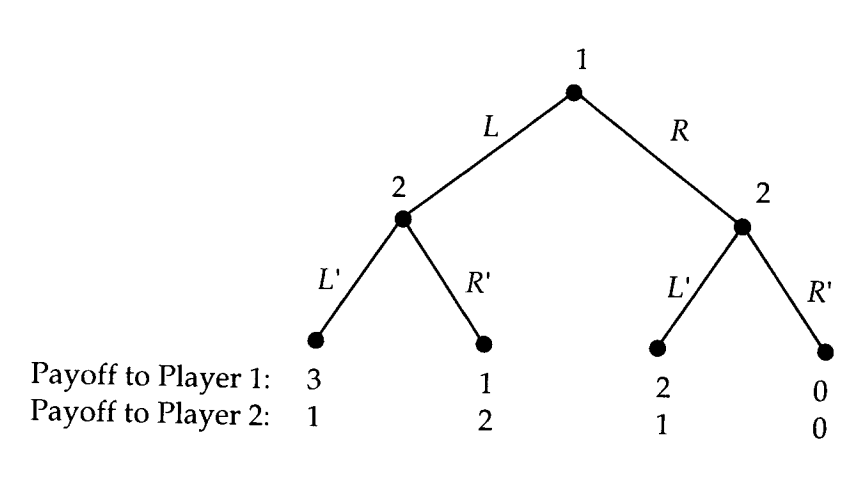
\includegraphics[width=0.6\textwidth]{arbol_juego.png}
    \caption{Árbol del juego dinámico}
    \label{fig:arbol_juego}
\end{figure}

\end{tcolorbox}

\usepackage[most]{tcolorbox}
\begin{tcolorbox}[colback=blue!10, title=Ejemplo 2, breakable] 
\textbf{Ejemplo 2} \\

Un monopolista (M) en un mercado que genera beneficios de 100 millones de dólares se enfrenta a la posibilidad de que un competidor (E) entre en el mercado. En primer lugar, el competidor decide si entrar (I) o no entrar (O) en el mercado.

Si el competidor entra en el mercado, el monopolista observa la acción del entrante y decide si luchar (F) o acomodar (A) al competidor. Si el monopolista lucha, se inicia una guerra de precios. Como resultado, ambas empresas terminan perdiendo 50 millones de dólares cada una. Si el monopolista acomoda, ambas empresas comparten el mercado a partes iguales. Supóngase que no hay costes de entrada para el competidor.

Podemos representar esta situación mediante un árbol de juego.

\begin{figure}[H]
    \centering
    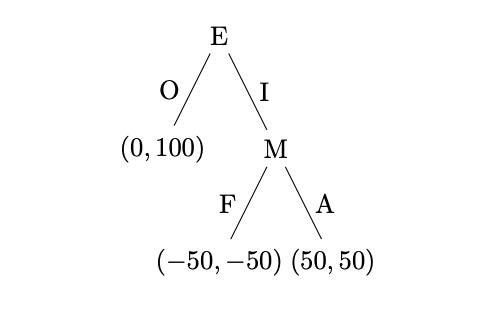
\includegraphics[width=0.6\textwidth]{arbol_juego2.png}
    \caption{Árbol de decisión de entrada de mercado con un monopolista y un competidor}
    \label{fig:arbol_juego}
\end{figure}

En el ejemplo anterior, vemos que el árbol de juego contiene toda la información relevante de la situación, a saber:
\begin{enumerate}
\item Los jugadores.

\item Las decisiones secuenciales posibles de los jugadores.

\item La información que conocen los jugadores.

\item Los pagos de los jugadores.
\end{enumerate}

El conjunto de estrategias de los jugadores es \(S_1 = \{O, I\},\; S_2 = \{F, A\}\). El juego puede representarse mediante la tabla

\begin{table}[H]
\centering
\begin{tabular}{c|cc}
 & \multicolumn{2}{c}{\textbf{Monopolista (M)}} \\
\textbf{Competidor (E)} & A & F \\ 
\hline
I & (50,50) & (-50,-50) \\
O & (0,100) & (0,100)
\end{tabular}
\caption{Forma normal del juego entre un monopolista y un competidor}
\label{tab:monopolio}
\end{table}

\end{tcolorbox}

\bibliography{bib/library.bib,bib/paquetes.bib}


%


\end{document}
